% Options for packages loaded elsewhere
\PassOptionsToPackage{unicode}{hyperref}
\PassOptionsToPackage{hyphens}{url}
\documentclass[
]{article}
\usepackage{xcolor}
\usepackage[margin=1in]{geometry}
\usepackage{amsmath,amssymb}
\setcounter{secnumdepth}{-\maxdimen} % remove section numbering
\usepackage{iftex}
\ifPDFTeX
  \usepackage[T1]{fontenc}
  \usepackage[utf8]{inputenc}
  \usepackage{textcomp} % provide euro and other symbols
\else % if luatex or xetex
  \usepackage{unicode-math} % this also loads fontspec
  \defaultfontfeatures{Scale=MatchLowercase}
  \defaultfontfeatures[\rmfamily]{Ligatures=TeX,Scale=1}
\fi
\usepackage{lmodern}
\ifPDFTeX\else
  % xetex/luatex font selection
\fi
% Use upquote if available, for straight quotes in verbatim environments
\IfFileExists{upquote.sty}{\usepackage{upquote}}{}
\IfFileExists{microtype.sty}{% use microtype if available
  \usepackage[]{microtype}
  \UseMicrotypeSet[protrusion]{basicmath} % disable protrusion for tt fonts
}{}
\makeatletter
\@ifundefined{KOMAClassName}{% if non-KOMA class
  \IfFileExists{parskip.sty}{%
    \usepackage{parskip}
  }{% else
    \setlength{\parindent}{0pt}
    \setlength{\parskip}{6pt plus 2pt minus 1pt}}
}{% if KOMA class
  \KOMAoptions{parskip=half}}
\makeatother
\usepackage{graphicx}
\makeatletter
\newsavebox\pandoc@box
\newcommand*\pandocbounded[1]{% scales image to fit in text height/width
  \sbox\pandoc@box{#1}%
  \Gscale@div\@tempa{\textheight}{\dimexpr\ht\pandoc@box+\dp\pandoc@box\relax}%
  \Gscale@div\@tempb{\linewidth}{\wd\pandoc@box}%
  \ifdim\@tempb\p@<\@tempa\p@\let\@tempa\@tempb\fi% select the smaller of both
  \ifdim\@tempa\p@<\p@\scalebox{\@tempa}{\usebox\pandoc@box}%
  \else\usebox{\pandoc@box}%
  \fi%
}
% Set default figure placement to htbp
\def\fps@figure{htbp}
\makeatother
% definitions for citeproc citations
\NewDocumentCommand\citeproctext{}{}
\NewDocumentCommand\citeproc{mm}{%
  \begingroup\def\citeproctext{#2}\cite{#1}\endgroup}
\makeatletter
 % allow citations to break across lines
 \let\@cite@ofmt\@firstofone
 % avoid brackets around text for \cite:
 \def\@biblabel#1{}
 \def\@cite#1#2{{#1\if@tempswa , #2\fi}}
\makeatother
\newlength{\cslhangindent}
\setlength{\cslhangindent}{1.5em}
\newlength{\csllabelwidth}
\setlength{\csllabelwidth}{3em}
\newenvironment{CSLReferences}[2] % #1 hanging-indent, #2 entry-spacing
 {\begin{list}{}{%
  \setlength{\itemindent}{0pt}
  \setlength{\leftmargin}{0pt}
  \setlength{\parsep}{0pt}
  % turn on hanging indent if param 1 is 1
  \ifodd #1
   \setlength{\leftmargin}{\cslhangindent}
   \setlength{\itemindent}{-1\cslhangindent}
  \fi
  % set entry spacing
  \setlength{\itemsep}{#2\baselineskip}}}
 {\end{list}}
\usepackage{calc}
\newcommand{\CSLBlock}[1]{\hfill\break\parbox[t]{\linewidth}{\strut\ignorespaces#1\strut}}
\newcommand{\CSLLeftMargin}[1]{\parbox[t]{\csllabelwidth}{\strut#1\strut}}
\newcommand{\CSLRightInline}[1]{\parbox[t]{\linewidth - \csllabelwidth}{\strut#1\strut}}
\newcommand{\CSLIndent}[1]{\hspace{\cslhangindent}#1}
\setlength{\emergencystretch}{3em} % prevent overfull lines
\providecommand{\tightlist}{%
  \setlength{\itemsep}{0pt}\setlength{\parskip}{0pt}}
\usepackage{bookmark}
\IfFileExists{xurl.sty}{\usepackage{xurl}}{} % add URL line breaks if available
\urlstyle{same}
\hypersetup{
  pdftitle={Modified Beta-Function Selection Model},
  hidelinks,
  pdfcreator={LaTeX via pandoc}}

\title{Modified Beta-Function Selection Model}
\author{}
\date{\vspace{-2.5em}}

\begin{document}
\maketitle

Selection models comprises two components. The first component,
hereinafter termed the \emph{evidence-generating process}, models the
distribution of effect sizes before selection, typically using a
conventional random-effects model or meta-regression model. The second
component, hereinafter termed the \emph{selection process}, identifies
how the distribution is changed based on the likelihood of an effect
size being reported. The combined model provides parameter estimates
that define the selection process, along with meta-analytic estimates
that are adjusted for selective reporting.

Following the approach outlined in our previous work on step-function
models (Pustejovsky, Citkowicz, and Joshi 2025), we model the
\emph{marginal} distribution of effect size estimates rather than the
joint distribution within studies. To account for dependence among
effect sizes, we use cluster-robust variance estimation or clustered
bootstrap methods, which accommodate within-study correlation without
requiring explicit modeling of the dependence structure. While this
strategy limits interpretation to the marginal distribution and does not
distinguish between study-level and outcome-level selection, it remains
a practical and plausible framework for modeling selective reporting
based on the significance of individual estimates.

We use the following notation to describe the model and estimation
procedures. Consider a meta-analytic dataset comprising \(J\) studies,
where study \(j\) reports \(k_j\) effect size estimates. Let \(y_{ij}\)
denote the \(i\)th effect size estimate from study \(j\), with
associated standard error \(\sigma_{ij}\) and one-sided \(p\)-value
\(p_{ij}\). The one-sided \(p\)-value is defined relative to the null
hypothesis that the true effect size is less than or equal to zero, with
alternative hypothesis that the effect size is positive. Let
\(\mathbf{x}_{ij}\) be a \(1 \times x\) row vector of predictors
representing characteristics of the effect size, sample, or study
procedures. We use \(\Phi()\) to denote the standard normal cumulative
distribution function and \(\phi()\) to denote the standard normal
density function.

\subsection{Evidence-generating
process}\label{evidence-generating-process}

We assume an evidence-generating process based on a standard
random-effects meta-regression model. Let \(Y^*\) denote a potentially
reported effect size estimate, with standard error \(\sigma^*\),
one-sided \(p\)-value \(p^*\), and predictor vector \(\mathbf{x}^*\).
Then the evidence-generating process is defined as \begin{equation}
\label{eq:meta-mean-regression}
\left(Y^* | \sigma^*, \mathbf{x}^*\right) \sim N\left(\mathbf{x}^* \boldsymbol\beta, \ \tau^2 + \sigma^{*2}\right),
\end{equation} where \(\boldsymbol\beta\) is an \(x \times 1\) vector of
regression coefficients and \(\tau^2\) is the marginal variance of the
effect size distribution. This model treats effect sizes as independent
and characterizes \emph{total} heterogeneity without decomposing within-
and between-study variation.

\subsection{Selection process}\label{selection-process}

A \(p\)-value selection process is defined by a selection function that
specifies the probability that an effect size is reported, conditional
on its \(p\)-value. Let \(O\) indicate whether \(Y^*\) is observed. The
process implies that \begin{equation}
\label{eq:selection-process}
\Pr\left(O = 1 | p^* \right) \propto w\left(p^*; \boldsymbol\lambda \right)
\end{equation} where \(w\left(.; \boldsymbol\lambda\right)\) is a known,
strictly positive function on the interval \([0, 1]\) with an unknown
\(h \times 1\) parameter vector \(\boldsymbol\lambda\).

Citkowicz and Vevea (2017) defined the selection function using a
truncated beta density with two parameters, offering flexibility to
capture diverse selection patterns more parsimoniously than the step
function model. Because the beta density can be unbounded near 0 and 1,
they proposed truncating it to make the model computationally tractable,
assuming constant selection probabilities for \(p\)-values in the range
\([0, \alpha_1]\) and \([\alpha_2, 1]\). Given these pre-specified
thresholds \(\alpha_1\) and \(\alpha_2\) and selection parameters
\(\boldsymbol\lambda = (\lambda_1, \lambda_2)\), the beta density
selection function is expressed by \begin{equation}
\label{eq:beta-density-p}
w(p^*_i, \boldsymbol\lambda) =  \begin{cases} 
\alpha_1^{\lambda_1 - 1} (1 - \alpha_1)^{\lambda_2 - 1} & \text{if} \quad p^*_i \leq \alpha_1 \\
\left(p^*_i\right)^{\lambda_1 - 1} (1 - p^*_i)^{\lambda_2 - 1} & \text{if} \quad \alpha_1 < p^*_i < \alpha_2 \\
\alpha_2^{\lambda_1 - 1} (1 - \alpha_2)^{\lambda_2 - 1} & \text{if} \quad \alpha_2 \leq p^*_i.
\end{cases}
\end{equation} Equation (\ref{eq:beta-density-p}) can be written
equivalently as \begin{equation}
\label{eq:beta-density-y}
w(Y^*_i / \sigma^*_i, \boldsymbol\lambda) =  \begin{cases} 
\alpha_1^{\lambda_1 - 1} (1 - \alpha_1)^{\lambda_2 - 1} & \text{if} \quad \sigma^*_i \Phi^{-1}(1 - \alpha_1) \leq Y^*_i \\
\left[\Phi\left(-Y^*_i / \sigma^*_i\right)\right]^{\lambda_1 - 1} \left[\Phi\left(Y^*_i / \sigma^*_i\right)\right]^{\lambda_2 - 1} & \text{if} \quad \sigma^*_i \Phi^{-1}(1 - \alpha_2) < Y^*_i < \sigma^*_i \Phi^{-1}(1 - \alpha_1) \\
\alpha_2^{\lambda_1 - 1} (1 - \alpha_2)^{\lambda_2 - 1} & \text{if} \quad  Y^*_i \leq \sigma^*_i \Phi^{-1}(1 - \alpha_2).
\end{cases}
\end{equation} When \(\lambda_1 = \lambda_2 = 1\), the selection
function is flat, the probability of selection does not depend on the
\(p\)-values, and selective reporting is absent.

Citkowicz and Vevea (Citkowicz and Vevea 2017) used extreme truncation
points (\(\alpha_1 = 10^{-5}\), \(\alpha_2 = 1 - 10^{-5}\)), but such
choices can make the model overly sensitive to rare, extreme
\(p\)-values, potentially producing implausible estimates (Hedges 2017).
Using more moderate, psychologically salient thresholds such as
\(\alpha_1 = .025\) and \(\alpha_2 = .975\) could potentially reduce
this sensitivity and yield more plausible selection patterns.

Figure @ref(fig:beta-functions) depicts several shapes that the beta
density can assume. Figure @ref(fig:beta-functions)a. presents a curve
in which there is preference for highly significant effects and the
probability of selection is strictly decreasing in the one-sided
p-value, where \(\lambda_1 = 0.5\) and \(\lambda_2 = 2.0\), and
thresholds of \(\alpha_1 = .025, \alpha_2 = .975\). Figure
@ref(fig:beta-functions)b. depicts a curve with \(\lambda_1 = 0.5\) and
\(\lambda_2 = 0.6\), a more complex form of selection in which both
significantly positive and significantly negative effect sizes are more
likely to be reported than null effects.

\begin{figure}[tb]
\subfloat[Decreasing selection: $\lambda_1 = 0.5, \lambda_2 = 2.0$\label{fig:beta-functions-1}]{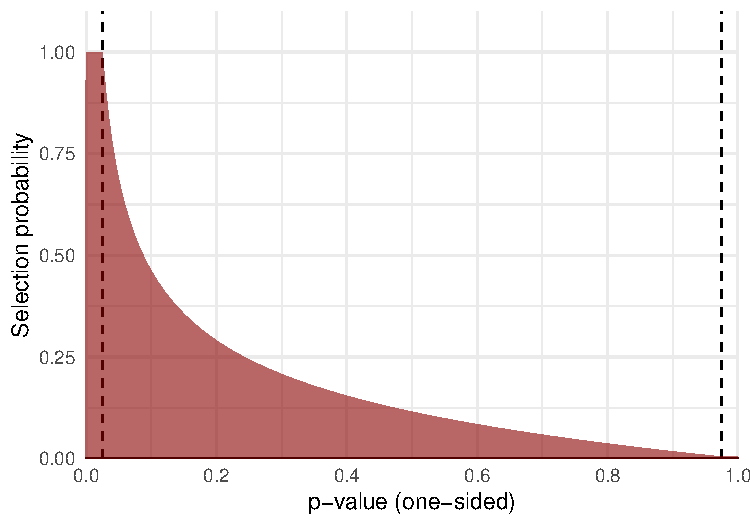
\includegraphics[width=0.49\linewidth]{model-and-estimation-methods_files/figure-latex/beta-functions-1} }\subfloat[Complex selection: $\lambda_1 = 0.5, \lambda_2 = 0.6$\label{fig:beta-functions-2}]{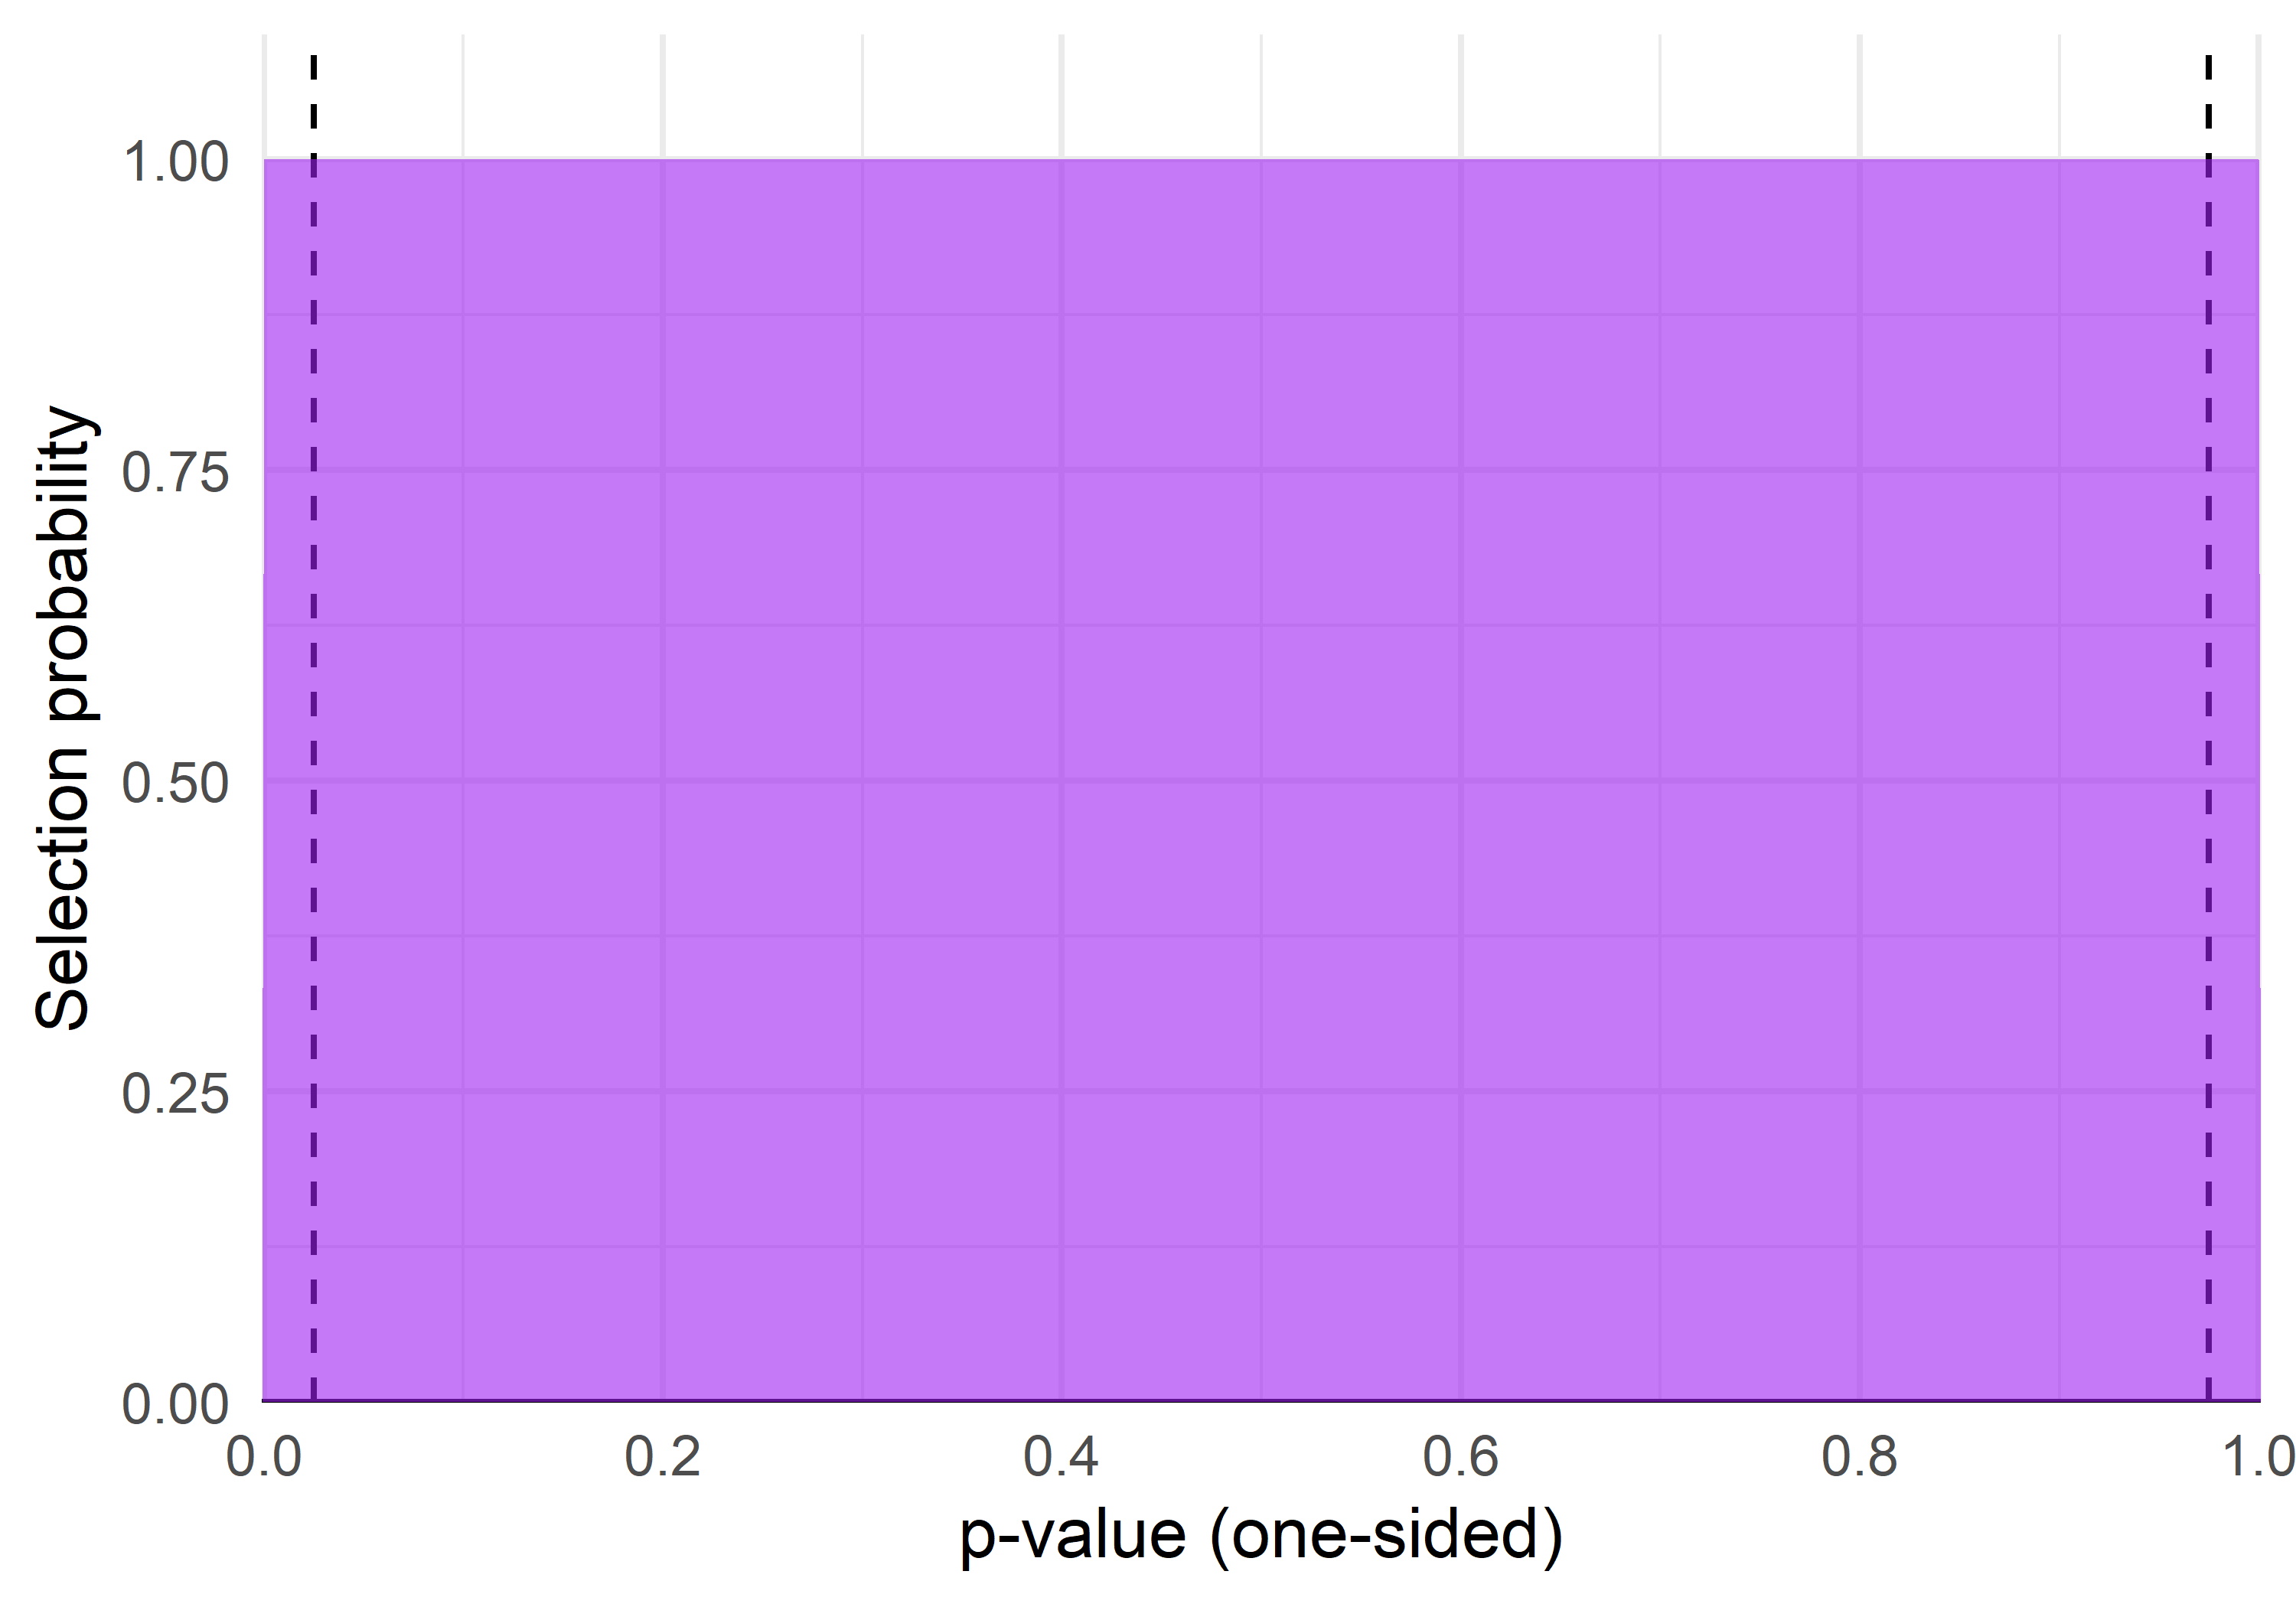
\includegraphics[width=0.49\linewidth]{model-and-estimation-methods_files/figure-latex/beta-functions-2} }\caption{Examples of beta density functions}\label{fig:beta-functions}
\end{figure}

\subsection{Distribution of observed effect size
estimates}\label{distribution-of-observed-effect-size-estimates}

The combined model for the marginal density of an observed effect size
estimate \(Y\) with standard error \(\sigma\) has the form
\begin{equation}
\label{eq:generic-selection}
f(Y = y | \sigma, \mathbf{x}) = \frac{1}{A(\mathbf{x}, \sigma; \boldsymbol\beta, \tau^2, \boldsymbol\lambda)} \times w\left(y, \sigma; \boldsymbol\lambda \right) \times \frac{1}{\sqrt{\tau^2 + \sigma^2}} \phi\left(\frac{y - \mathbf{x} \boldsymbol\beta}{\sqrt{\tau^2 + \sigma^2}}\right),
\end{equation} where \begin{equation}
\label{eq:generic-selection-A}
A(\mathbf{x}, \sigma; \boldsymbol\beta, \tau^2, \boldsymbol\lambda) =  \int_\mathbb{R} w\left(y, \sigma; \boldsymbol\lambda \right) \times  \frac{1}{\sqrt{\tau^2 + \sigma^2}}\phi\left(\frac{y - \mathbf{x}\boldsymbol\beta}{\sqrt{\tau^2 + \sigma^2}}\right) dy.
\end{equation} For the beta-function selection process, the
\(A(\mathbf{x}, \sigma; \boldsymbol\beta, \tau^2, \boldsymbol\lambda)\)
term in the beta-function composite likelihood must be computed using
numerical integration. If \(w(y, \sigma; \boldsymbol\lambda) = 1\), then
\(A(\mathbf{x}, \sigma; \boldsymbol\beta, \tau^2, \boldsymbol\lambda) = 1\)
and there is no selective reporting. The density then reduces to the
unweighted density of the evidence-generating process and the
\(\boldsymbol\beta\) estimates from the adjusted beta function selection
model will approximate those of the standard meta-analytic model.

\subsection{Estimation Method}\label{estimation-method}

We estimate model parameters using maximum composite marginal likelihood
(CML), which treats each observed effect size estimate as if it were
mutually independent, following established composite likelihood
approaches (e.g., Cox and Reid 2004; Lindsay 1988; Varin 2008).
Estimation proceeds by maximizing a weighted log-likelihood function
defined over the marginal contributions of each observation, using
reparameterizations of the variance and selection parameters. Confidence
intervals are constructed using robust (sandwich-type) variance
estimators based on study-level score contributions. A detailed
explanation of CML methods is provided in our previous paper
(Pustejovsky, Citkowicz, and Joshi 2025), and the exact expressions used
for estimating the beta-function selection model are presented in
APPENDIX.

\subsection{Bootstrap inference}\label{bootstrap-inference}

To improve inference accuracy with a limited number of studies, we also
implement bootstrap procedures, which generate pseudo-samples through
random resampling or reweighting of the original data. We consider both
the non-parametric clustered bootstrap and the fractional random weight
bootstrap (Xu et al. 2020), which differ in how they preserve the
dependence structure across clusters. Confidence intervals are then
computed using standard bootstrap-based methods such as the percentile,
basic, studentized, and bias-corrected-and-accelerated intervals
(Davison and Hinkley 1997; Efron 1987). These resampling-based
procedures are particularly useful in small-sample contexts where
sandwich estimators may perform poorly. APPENDIX provides further
details about the bootstrap CI calculations.

\protect\phantomsection\label{refs}
\begin{CSLReferences}{1}{0}
\bibitem[\citeproctext]{ref-citkowicz2017parsimonious}
Citkowicz, Martyna, and Jack L Vevea. 2017. {``{A parsimonious weight
function for modeling publication bias}.''} \emph{Psychological Methods}
22 (1): 28--41. \url{https://doi.org/10.1037/met0000119}.

\bibitem[\citeproctext]{ref-cox2004note}
Cox, D. R., and N. Reid. 2004. {``A Note on Pseudolikelihood Constructed
from Marginal Densities.''} \emph{Biometrika} 91 (3): 729--37.
\url{https://doi.org/10.1093/biomet/91.3.729}.

\bibitem[\citeproctext]{ref-davison1997bootstrap}
Davison, A. C., and D. V. Hinkley. 1997. \emph{Bootstrap Methods and
Their Applications}. Cambridge: Cambridge University Press.

\bibitem[\citeproctext]{ref-efron1987better}
Efron, Bradley. 1987. {``Better Bootstrap Confidence Intervals.''}
\emph{Journal of the American Statistical Association} 82 (397):
171--85. \url{https://doi.org/10.1080/01621459.1987.10478410}.

\bibitem[\citeproctext]{ref-hedges2017plausibility}
Hedges, Larry V. 2017. {``Plausibility and Influence in Selection
Models: {A} Comment on {Citkowicz} and {Vevea} (2017).''}
\emph{Psychological Methods} 22 (1): 42--46.
\url{https://doi.org/10.1037/met0000108}.

\bibitem[\citeproctext]{ref-lindsay1988composite}
Lindsay, Bruce G. 1988. {``Composite Likelihood Methods.''} In
\emph{Contemporary {Mathematics}}, edited by N. U. Prabhu, 80:221--39.
Providence, Rhode Island: American Mathematical Society.
\url{https://doi.org/10.1090/conm/080/999014}.

\bibitem[\citeproctext]{ref-pustejovsky2025step}
Pustejovsky, James E., Martyna Citkowicz, and Megha Joshi. 2025.
{``Estimation and Inference for Step-Function Selection Models in
Meta-Analysis with Dependent Effects.''} \emph{Journal Name}.

\bibitem[\citeproctext]{ref-varin2008composite}
Varin, Cristiano. 2008. {``On Composite Marginal Likelihoods.''}
\emph{AStA Advances in Statistical Analysis} 92 (1): 1--28.
\url{https://doi.org/10.1007/s10182-008-0060-7}.

\bibitem[\citeproctext]{ref-xu2020applications}
Xu, Li, Chris Gotwalt, Yili Hong, Caleb B King, and William Q Meeker.
2020. {``Applications of the Fractional-Random-Weight Bootstrap.''}
\emph{The American Statistician} 74 (4): 345--58.
\url{https://doi.org/10.1080/00031305.2020.1731599}.

\end{CSLReferences}

\end{document}
